\def\Ponderation{40}
\def\SigleNumero{STT-1000}
\def\NomCours{Probabilités et statistique}
\def\DateEvaluation{30 avril 2026}
\def\HeureEvaluation{18 h 30 à 21 h 20}
\def\Session{}
\def\NomEvaluation{Examen 2}

% Ne rien mettre entre les accolades si l'enseignant (ou l'enseignante) est aussi le coordonnateur (ou la coordonnatrice)
\def\Coordonnatrice{}
\def\Coordonnateur{}

% Ne rien mettre entre les accolades s'il y a plus d'une section
\def\Enseignant{}
\def\Enseignante{}

% Ne rien mettre entre les accolades s'il s'agit d'un cours à section unique
% Mettre le nom de chacun des enseignants et enseignantes entre les accolades
% Une case à cocher sera générée pour chacune des sections
\def\SectionA{Anne-Sophie Charest}
\def\SectionB{Julien Miron}
\def\SectionC{}
\def\SectionD{}


\def\Directives{
\begin{enumerate}
\item Matériel autorisé:
\begin{itemize}
\item Calculatrice scientifique {\bf autorisée par la faculté des sciences et de génie};
\item Le feuillet de formules fourni avec l'examen. Celui-ci inclut la table de la loi normale. Veuillez ne rien écrire sur le feuillet de formules.
\end{itemize}
\item Assurez-vous que cette évaluation comporte \numquestions ~exercices répartis sur \numpages{}~pages, pour un total de \numpoints{}~points.\
\item \textbf{Veuillez ne pas dégrafer votre examen.}
\item Vous devez\textbf{ justifier toutes vos réponses} par une démarche claire, sauf pour les questions à choix de réponse.\
\item Pour les questions à choix de réponse et les vrais ou faux, vous pouvez mettre un X, un crochet ($\checkmark$) ou remplir la case.\
\item Vous devez laisser tout ce qui ne servira pas durant l'examen à l'avant de la salle AVANT de rejoindre votre place.\
\item Vous n'avez droit à AUCUN appareil électronique en votre possession durant l'examen.
\item Une fois assis à votre place, vous devez demandez l'autorisation pour vous lever, même si l'examen n'est pas encore commencé, sauf lorsque vous avez terminé l'examen.
\item Dans les 5 dernières minutes de l'examen, il sera interdit de se lever avant que TOUTES les copies n'aient été ramassées.
\end{enumerate}
\begin{itemize}
\item[$\rightarrow$] Le non-respect des consignes 7-8-9 entraînera une pénalité de 10\%.
\end{itemize}
Attention, la formule correcte pour les degrés de liberté $\nu$ est 
$$\nu = \frac{(s_1^2/n_1 + s^2_2/n_2)^2}{ \frac{(s_1^2/n_1)^2}{n_1 +1} + \frac{(s^2_2/n_2)^2}{n_2 + 1} } -2 $$
}

\providecommand{\Gradescope}{}


\documentclass{Evaluation}
\usepackage{multicol,graphicx}

\noprintanswers
\begin{document}

\begin{questions}


\pageblanche

%%%%%%%%%%%%%%%% QUESTIONS MODULES 1 à 5 %%%%%%%%%%%%%%%%

\question[4]
Soit deux événements $A$ et $B$ formant une partition de l'espace, avec $P(A)=0,7$. \\On a aussi que $P(D\mid A)=0,02$, $P(D\mid B)=0,05$.

Quelle expression permet de calculer $P(B\mid D)$ ?

\begin{checkboxes}
\choice $\dfrac{0,3\times 0,05}{0,02 + 0,05}$
\choice $\dfrac{0,05}{0,7\times 0,02 + 0,3\times 0,05}$
\choice $\dfrac{0,7\times 0,02}{0,7\times 0,02 + 0,3\times 0,05}$
\correctchoice $\dfrac{0,3\times 0,05}{0,7\times 0,02 + 0,3\times 0,05}$
\choice $\dfrac{0,3\times 0,05}{0,7\times 0,02 + 0,7\times 0,05}$
\end{checkboxes}


\question[3]
Une file de clients arrive selon un processus de Poisson de taux $2$ par heure. On s’intéresse au temps d’attente jusqu’au prochain client. Quelle est l’expression correcte pour calculer la probabilité que ce temps soit inférieur à $1$ heure?


\begin{checkboxes}
\correctchoice $P(T\leq 1)$, où $T\sim \mathrm{Exp}(2)$
\choice $P(T=1)$, où $T\sim \mathrm{Exp}(2)$
\choice $P(X=1)$, où $X\sim \mathrm{Poisson}(2)$
\choice $P(X\leq 1)$, où $X\sim \mathrm{Poisson}(2)$
\choice $P(T\leq 1)$, où $T\sim \mbox{Gamma}(2,2)$
\end{checkboxes}


\begin{solution}
La bonne réponse est \textbf{a)}.

Dans un processus de Poisson de taux $2$ par heure, le \textbf{temps d’attente jusqu’au prochain événement} suit une loi exponentielle de paramètre $2$. On doit donc utiliser
$$
P(T\leq 1), \qquad T\sim \mathrm{Exp}(2).
$$

Problèmes avec les autres réponses : 
\begin{itemize}
\item \textbf{c)} et \textbf{d)} utilisent une loi de Poisson, qui sert à modéliser un \emph{nombre} d’événements dans un intervalle de temps, et non un temps d’attente;
\item \textbf{b)} utilise une probabilité ponctuelle pour une variable continue;
\item \textbf{e)} la loi gamma conviendrait au temps d’attente jusqu’au \emph{deuxième} client, pas jusqu’au prochain.
\end{itemize}
\end{solution}




\question[4]
Soit la loi conjointe de $X$ et $Y$ :

$$
\begin{array}{c|cc}
 & Y=0 & Y=1 \\
\hline
X=0 & 0{,}2 & 0{,}3 \\
X=1 & 0{,}1 & 0{,}4 \\
\end{array}
$$

Quelle est la valeur de $P(Y=1 \mid X=1)$? Laissez des traces de votre démarche.


\begin{solution}
$$
P(Y=1 \mid X=1)=\frac{P(X=1,Y=1)}{P(X=1)}=\frac{0{,}4}{0{,}1+0{,}4}=0{,}8
$$
\end{solution}

%%%%%%%%%%%%%%%% STATISTIQUES DESCRIPTIVES %%%%%%%%%%%%%%%%

%%%%%%%%%%%%%%%% LOIS ÉCHANTILLONNALES %%%%%%%%%%%%%%%%

%%%%%%%%%%%%%%%% INTERVALLES DE CONFIANCE %%%%%%%%%%%%%%%%

\pageblanche

\question[]

\begin{parts}

\part[6]
On compare le temps moyen (en millisecondes) nécessaire pour exécuter une même tâche avec deux algorithmes.

\begin{itemize}
\item Algorithme A : $n_1=50$, $\bar x_1=72$, $s_1=10$
\item Algorithme B : $n_2=60$, $\bar x_2=65$, $s_2=12$
\end{itemize}

On suppose que les temps d’exécution suivent des lois normales avec variances inconnues mais égales.

Construisez un intervalle de confiance à 95 \% pour la différence des moyennes $\mu_A - \mu_B$.

\begin{solution}
On utilise l’intervalle de confiance avec variance poolée.

$$
s_p^2 = \frac{(n_1-1)s_1^2 + (n_2-1)s_2^2}{n_1+n_2-2}
= \frac{49\times100 + 59\times144}{108}
= \frac{13396}{108} \approx 124{,}04
$$

$$
s_p \approx 11{,}14
$$

$$
SE = s_p \sqrt{\frac{1}{n_1}+\frac{1}{n_2}}
= 11{,}14 \sqrt{\frac{1}{50}+\frac{1}{60}}
\approx 2{,}13
$$

ddl $= 108$, donc $t_{0{,}975} \approx 1{,}98$

$$
(\bar x_1-\bar x_2) \pm t \cdot SE
= 7 \pm 1{,}98 \times 2{,}13
\approx 7 \pm 4{,}22
$$

Intervalle de confiance :
$$
[2{,}78 \; ; \; 11{,}22]
$$
\end{solution}
\vfill

\part
\begin{subparts}
        \subpart[1] L'intervalle à 90\% aurait été plus court.
        
        \begin{oneparcheckboxes}
            \correctchoice Vrai
            \choice Faux
        \end{oneparcheckboxes}

        \subpart[1] Puisque les tailles d'échantillons sont grandes, cet intervalle est valide même sans l'hypothèse de normalité des observations.
        
        \begin{oneparcheckboxes}
            \choice Vrai
            \correctchoice Faux
        \end{oneparcheckboxes}

    \end{subparts}
\end{parts}

\pageblanche

\question[]

\begin{parts}

\part[7]
On souhaite estimer la proportion d’élèves du secondaire qui utilisent l’intelligence artificielle pour faire leurs travaux scolaires. On veut construire un intervalle de confiance de niveau 90 \% pour cette proportion, avec une marge d’erreur d’au plus 0,04. Quelle taille d’échantillon minimale faut-il utiliser?

\begin{solution}
Pour un intervalle de confiance pour une proportion, la marge d’erreur vaut
$$
z_{0,95}\sqrt{\frac{\hat p(1-\hat p)}{n}}.
$$

Comme on ne connaît pas la valeur de la proportion, on prend le cas le plus défavorable, soit
$$
\hat p(1-\hat p)=0,25.
$$

On veut donc
$$
z_{0,95}\sqrt{\frac{0,25}{n}} \leq 0,04.
$$

Comme $z_{0,95}\approx 1{,}645$, on obtient
$$
1{,}645\sqrt{\frac{0,25}{n}} \leq 0,04.
$$

Donc
$$
\sqrt{\frac{0,25}{n}} \leq \frac{0,04}{1{,}645},
$$
puis
$$
\frac{0,25}{n} \leq \left(\frac{0,04}{1{,}645}\right)^2.
$$

Ainsi,
$$
n \geq \frac{0,25}{(0{,}04/1{,}645)^2} \approx 422{,}82.
$$

Il faut donc prendre au minimum
$$
\boxed{423}
$$
élèves.
\end{solution}

\vfill
\part[2]
Le directeur de l'école souhaite plutôt une marge d'erreur d'au plus $0,02$. Est-ce que la taille d'échantillon proposée en (a) est suffisante pour ce faire?

\begin{oneparcheckboxes}
\choice Oui, car la taille d’échantillon dépend seulement du niveau de confiance. \\
\choice Oui, car la marge d’erreur diminue quand la proportion est plus petite. \\
\choice Non, car le niveau de confiance est trop élevé. \\
\correctchoice Non, il faudrait augmenter la taille d’échantillon.
\end{oneparcheckboxes}
        
\end{parts}

\pageblanche
\question[3]

On construit un intervalle de confiance à 95 \% pour la variance d'une loi normale.
$[4 \; ; \; 16]$.

Parmi les affirmations suivantes, cochez toutes celles qui sont correctes.

\begin{oneparcheckboxes}
\choice La variance a 95 \% de probabilité d’être entre 4 et 16.\\
\correctchoice Si on répétait l’échantillonnage, environ 95 \% des intervalles construits contiendraient la vraie variance.\\
\correctchoice Une valeur de 12 est plausible pour la variance de la population.\\
\choice La variance observée dans l'échantillon est égale à 10.\\
\choice 95 \% des observations sont comprises entre 4 et 16.\\
\correctchoice Un test d'hypothèse bilatéral avec $\alpha = 0.05$ rejetterait l'hypothèse $H_0 : \sigma^2 = 20$.
\end{oneparcheckboxes}

\question[4]
Soient $X \sim \mathcal{N}(10, 4)$ et $Y \sim \mathcal{N}(5, 1)$, deux variables aléatoires indépendantes. \\
On définit $Z = 2X - Y$. Quelle est la loi de $Z$? Laissez des traces de votre démarche.


\begin{solution}
On utilise les propriétés des combinaisons linéaires de variables normales indépendantes.

$$
\mathbb{E}(Z) = 2\mathbb{E}(X) - \mathbb{E}(Y) = 2(10) - 5 = 15
$$

$$
\mathrm{Var}(Z) = 4\mathrm{Var}(X) + \mathrm{Var}(Y) = 4(4) + 1 = 17
$$

Donc
$$
Z \sim \mathcal{N}(15, 17).
$$

\end{solution}
%%%%%%%%%%%%%%%% TESTS D'HYPOTHÈSES %%%%%%%%%%%%%%%%

%%%%%%%%%%%%%%%% RLS %%%%%%%%%%%%%%%%

\pageblanche

\question\label{rls}

On étudie la relation entre le nombre d'heures passées à pratiquer un logiciel de programmation
($x$, en heures) et le score obtenu à un test ($y$, en points) chez $n=12$ élèves.

Un modèle de régression linéaire simple a été ajusté. On obtient :
$$
\hat y = 41{,}3 + 2{,}6x,
\qquad
\hat\sigma^2 = 4,
\qquad
S_{xx}=25.
\qquad S_{yy}=200.
$$


\begin{parts}
\part[3] Pour une observation donnée, on a $x=4$ et $y=53$.
Calculez le résidu associé à cette observation.


\begin{solution}
$$
\hat y = 41{,}3 + 2{,}6 \times 4 = 51{,}7
$$

$$
e = y - \hat y = 53 - 51{,}7 = 1{,}3
$$

\end{solution}
\vspace{6cm}

\part[6] 
Au seuil 5 \%, peut-on affirmer qu'il y a un lien linéaire entre le temps d'étude et le score obtenu au test?



\begin{solution}
On peut utiliser un test d'hypothèse ou un intervalle de confiance.

Test d'hypothèse : 

$$
H_0:\beta_1=0
\qquad \text{contre} \qquad
H_1:\beta_1\neq 0
$$


On a
$$
\hat\beta_1=2{,}6,
\qquad
\hat\sigma^2=4,
\qquad
S_{xx}=25,
\qquad
n=12.
$$

L'erreur-type de $\hat\beta_1$ est
$$
\sqrt{\frac{\hat\sigma^2}{S_{xx}}}
=
\sqrt{\frac{4}{25}}
=
0{,}4.
$$

La statistique de test est donc
$$
T_0=
\frac{\hat\beta_1-0}{\sqrt{\hat\sigma^2/S_{xx}}}
=
\frac{2{,}6}{0{,}4}
=
6{,}5.
$$

Sous $H_0$, on a
$$
T_0 \sim t_{n-2}=t_{10}.
$$

Pour un test bilatéral au seuil $\alpha=0{,}05$, la région de rejet est
$$
|T_0|>t_{1-\alpha/2,\,10}=t_{0{,}975,\,10}\approx 2{,}228.
$$

Comme
$$
|6{,}5|>2{,}228,
$$
on rejette $H_0$.

Il y a donc une relation linéaire significative entre $x$ et $y$ au seuil de $5\%$.

\vspace{0.5em}

Intervalle de confiance : 

Un intervalle de confiance à $95\%$ pour $\beta_1$ est
$$
\hat\beta_1 \pm t_{0{,}975,\,10}\sqrt{\frac{\hat\sigma^2}{S_{xx}}}
=
2{,}6 \pm 2{,}228(0{,}4).
$$

Ainsi,
$$
IC_{95\%}(\beta_1)
=
2{,}6 \pm 0{,}8912
=
[1{,}7088,\; 3{,}4912].
$$

Comme $0$ n'appartient pas à cet intervalle, cela concorde avec le rejet de $H_0$.

\end{solution}

\vfill
\pagesuivante{\ref{rls}}
\part[3]
Calculez le coefficient de détermination $R^2$ et interprétez le dans le contexte.
\begin{solution}
On utilise la formule
$$
R^2 = \hat\beta_1^2 \frac{S_{xx}}{S_{yy}}.
$$

$$
R^2 = (2{,}6)^2 \times \frac{25}{200}
= 6{,}76 \times 0{,}125
= 0{,}845.
$$

Donc
$$
R^2 \approx 0{,}85.
$$

Interprétation : environ 85 \% de la variabilité du score obtenu est expliqué par le nombre d'heures passées à pratiquer le logiciel.
\end{solution}
\end{parts}


\vspace{8cm}




\question[3]

Parmi les graphiques ci-dessous, lequel illustre un problème avec l'homogénéité de la variance des erreurs d'un modèle de régression linéaire simple. Cochez la bonne réponse.\\

\begin{oneparcheckboxes}
\choice A 
\correctchoice B
\choice C
\choice D
\end{oneparcheckboxes}

\begin{center}
\includegraphics[scale=0.7]{diagRLS.png}
\end{center}


\pageblanche

\question
Une entreprise fabrique des palettes de chocolat et s'intéresse à la variabilité de la quantité de sucre dans une palette. Elle choisit au hasard 11 palettes. Dans l'échantillon, la quantité moyenne de sucre par palette est de $20,05 \,g$ et la variance échantillonnale est de $7,995\, g^2$. Sachant que $X$, la quantité de sucre dans une palette, est une variable aléatoire qui suit une loi normale d'espérance $\mu$ et de variance $\sigma^2$, elle fait le test suivant, au seuil $\alpha=2,5\%$,
\begin{align*}
	H_0 &: \sigma^2 = 5 \cr
	H_1 &: \sigma^2 > 5.
\end{align*}

\begin{parts}
\part[3] Quelle est la valeur critique du test en grammes$^2$, c'est-à-dire, à partir de quelle valeur de $S^2$ rejette-t-on~$H_0$?

\begin{oneparcheckboxes}
    \choice 1,960
    \choice 2,131
    \CorrectChoice 10,24
    \choice 15,99
    \choice 20,48
\end{oneparcheckboxes} 

\vspace{1cm}
\part[2] Quelle est la valeur de la statistique du test sous $H_0$, arrondie à 3 décimales?

\begin{oneparcheckboxes}
    \choice 1,960
    \choice 2,131
    \choice 10,24
    \CorrectChoice 15,99
    \choice 20,48
\end{oneparcheckboxes} 

\begin{solution}
On sait que la statistique du test est $U_0=(n-1)S^2/\sigma^2_0$. Donc $U_0=10*7,995/5=15,99.$
\end{solution}

\vspace{1cm}
\part[2] Quel est le seuil observé du test?

	\begin{checkboxes}
	    \choice $\alpha^*=0,01$.
		\choice $\alpha^*=0,025$.
		\choice $\alpha^*=0,05$ .
		\CorrectChoice $\alpha^* =0,1$.
	\end{checkboxes}

\vspace{1cm}
\part[3] Si en réalité $\sigma^2=6,4$ et que la règle de décision est de rejeter $H_0$ si $\displaystyle\frac{10S^2}{5}>20,48$, quelle est l'expression de la puissance du test? 

\begin{checkboxes}
    \choice $P\left(\displaystyle \frac{10S^2}{5,1}>20,48\right)$
    \choice $P\left(\displaystyle \frac{10S^2}{5}>20,48\right)$
    \correctchoice $P\left(\displaystyle \frac{10S^2}{5,1}>16\right)$
    \choice $P\left(\displaystyle \frac{10S^2}{5}>16\right)$
\end{checkboxes}

\end{parts}

\pageblanche
\question[10] Soit $X_1,\hdots,X_{4}$ et $Y_1,\hdots,Y_{3}$ deux échantillons aléatoires provenant respectivement de lois normales d'espérances $\mu_X$ et $\mu_Y$ et de variance $\sigma^2_X$ et $\sigma^2_Y$, supposées égales.
On veut procéder à un test de seuil $\alpha$ avec les hypothèses

\begin{align*}
    H_0:\mu_X-\mu_Y=0, & & H_1:\mu_X-\mu_Y>0.
\end{align*}

On obtient $\overline{x}=26,112$, $\overline{y}=12$, $s_X^2=25$ et $s_Y^2=15$. Quel est le seuil observé du test?

\begin{solution}
On utilise le test $t$ à deux échantillons avec variances égales. La variance pondérée est :
$$s_p^2=\frac{(n_X-1)s_X^2+(n_Y-1)s_Y^2}{n_X+n_Y-2}=\frac{3\times 25+2\times 15}{4+3-2}=\frac{75+30}{5}=\frac{105}{5}=21.$$
L'écart-type de la différence est :
$$se=s_p\sqrt{\frac{1}{n_X}+\frac{1}{n_Y}}=\sqrt{21}\times\sqrt{\frac{1}{4}+\frac{1}{3}}=\sqrt{21\times\frac{7}{12}}=\sqrt{\frac{147}{12}}=\sqrt{12{,}25}=3{,}5.$$
La statistique de test est :
$$t_0=\frac{\overline{x}-\overline{y}}{se}=\frac{26{,}112-12}{3{,}5}=\frac{14{,}112}{3{,}5}=4{,}032.$$
Les degrés de liberté sont $\nu=n_X+n_Y-2=5$. Le seuil observé est $\alpha^*=P(T_5>4{,}032)$. D'après la table de la loi $t$, $t_{0{,}01,\,5}=3{,}365$ et $t_{0{,}005,\,5}=4{,}032$. Puisque $t_0=4{,}032=t_{0{,}005,\,5}$, on a $\alpha^*=0{,}005$. On rejette $H_0$ au seuil $5\%$.
\end{solution}
\pageblanche
\question[10] Soit $X_1,\hdots, X_{n}$ qui proviennent d'une loi normale d'espérance $\mu$ et de variance $\sigma^2=25$. 
On fait le test d'hypothèses pour lequel $H_0:\mu=5$ et $H_1:\mu>5$ au seuil $\alpha=2,5\%$.
Pour quelles valeurs de $n$ rejette-t-on $H_0$ si $\overline{x}=5,1$?

\begin{solution}
    On rejette $H_0$ si 

    \begin{align*}
        Z_0&>1,96\\
        \frac{\overline{x}-5}{5/\sqrt{n}}&>1,96\\
        \sqrt{n}(\overline{x}-5)&>9,8\\
        \sqrt{n}&>\frac{9,8}{0,1}\\
        n&>9604
    \end{align*}
\end{solution}
\pageblanche

\question Dites si les énoncés suivants sont vrais ou faux.

\begin{parts}
    \part[1] Soit $x_1,\hdots,x_n$. Si la médiane échantillonnale est $25$, nous sommes certains que la valeur de l'observation du milieu est $25$.

    \begin{oneparcheckboxes}
        \choice Vrai
        \correctchoice Faux
    \end{oneparcheckboxes}

    \begin{solution}
    Faux. Si $n$ est pair, la médiane est la moyenne des deux observations centrales; aucune d'elles n'est forcément égale à $25$. Cette propriété n'est garantie que si $n$ est impair.
    \end{solution}

        \part[1] Soit $x_1,\hdots,x_n$. Si la moyenne échantillonnale est $25$, environ $50\%$ des observations sont plus grandes que $25$ et environ $50\%$ sont plus petites que $25$.

    \begin{oneparcheckboxes}
        \choice Vrai
        \correctchoice Faux
    \end{oneparcheckboxes}
    
    \begin{solution}
    Faux. C'est une propriété de la \textbf{médiane}, pas de la moyenne. La moyenne est sensible aux valeurs extrêmes et ne partage pas nécessairement l'échantillon en deux moitiés égales.
    \end{solution}

        \part[1] Soit $x_1,\hdots,x_n$. Si $Q_1=12$, nous savons que le minimum de l'échantillon est 12.

    \begin{oneparcheckboxes}
        \choice Vrai
        \correctchoice Faux
    \end{oneparcheckboxes}
 
    \begin{solution}
    Faux. $Q_1$ est le premier quartile (25\textsuperscript{e} percentile); le minimum de l'échantillon peut être strictement inférieur à $Q_1$.
    \end{solution}

        \part[1] Soit $x_1,\hdots,x_n$. Nous savons que $Q_3>0$.

    \begin{oneparcheckboxes}
        \choice Vrai
        \correctchoice Faux
    \end{oneparcheckboxes}

    \begin{solution}
    Faux. $Q_3$ dépend des données. Si toutes les observations sont négatives, $Q_3<0$.
    \end{solution}
    

\end{parts}

\vspace{0.5cm}
\question[3]
\noindent
\begin{minipage}[t]{0.5\linewidth}\vspace{0pt}
Soit l'histogramme ci-contre.

Dans quelle classe de l'histogramme se situe le quantile d'ordre 0,30?

\begin{checkboxes}
  \choice Dans la classe [10,15[
  \correctchoice Dans la classe [15,20[
  \choice Dans la classe [20,25[
  \choice Dans la classe [25,30[
  \choice Dans la classe [30,35[
\end{checkboxes}
\end{minipage}\hfill
\begin{minipage}[t]{0.42\linewidth}\vspace{0pt}
\centering
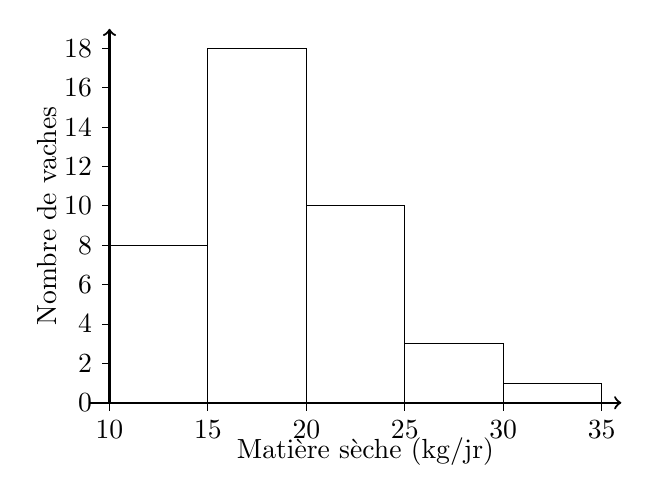
\begin{tikzpicture}[x=0.25cm,y=0.25cm]

% -------------------------------------------------
% Axes
% -------------------------------------------------
\draw[->, thick] (9,0) -- (36,0);   % axe x
\draw[->, thick] (10,0) -- (10,19); % axe y

% -------------------------------------------------
% Graduations x
% -------------------------------------------------
\foreach \x in {10,15,20,25,30,35}
  \draw (\x,0) -- (\x,-0.4) node[below] {\x};

% -------------------------------------------------
% Graduations y
% -------------------------------------------------
\foreach \y in {0,2,4,6,8,10,12,14,16,18}
  \draw (10,\y) -- (9.6,\y) node[left] {\y};

% -------------------------------------------------
% Labels
% -------------------------------------------------
\node at (23,-2.5) {Mati\`ere s\`eche (kg/jr)};
\node[rotate=90] at (6.8,9.5) {Nombre de vaches};

% -------------------------------------------------
% Histogramme
% -------------------------------------------------
\draw (10,0) rectangle (15,8);
\draw (15,0) rectangle (20,18);
\draw (20,0) rectangle (25,10);
\draw (25,0) rectangle (30,3);
\draw (30,0) rectangle (35,1);

\end{tikzpicture}
\end{minipage}

\begin{solution}
    Le nombre total de vaches est $8+18+10+3+1=40$. Le quantile d'ordre $0{,}30$ correspond à la position $0{,}30 \times 40 = 12$. L'effectif cumulé après la classe $[10,15[$ est $8$. L'effectif cumulé après la classe $[15,20[$ est $8+18=26$. Puisque $8 < 12 \leq 26$, le quantile d'ordre $0{,}30$ se situe dans la classe $[15,20[$.
\end{solution}

\question[3]
Dans un laboratoire de microtechnique, Benjamin et Guillaume ont étudié le temps de réaction (en millisecondes) d'un certain type de détecteur de mouvements. Les 21 valeurs suivantes sont des temps de réaction collectés au cours d'une journée:

\begin{center}
\begin{tabular}{  c c c c c c c c }
111  &111  &111  &112  &113  &113  &113 \\
113 &115  &115  &115  &115 &115 & 116 \\
116 & 118 & 118 & 119 & 125 &125 & 128\\
\end{tabular}
\end{center}

Le diagramme en boîte ci-dessous a été tracé à partir de ces résultats. Il manque toutefois quelque chose à ce diagramme (il ne s'agit pas d'un titre ou de noms d'axes).


Ajoutez \textbf{sur le diagramme} l'élément manquant et dites ce que vous avez fait sous le diagramme. 
\begin{center}
		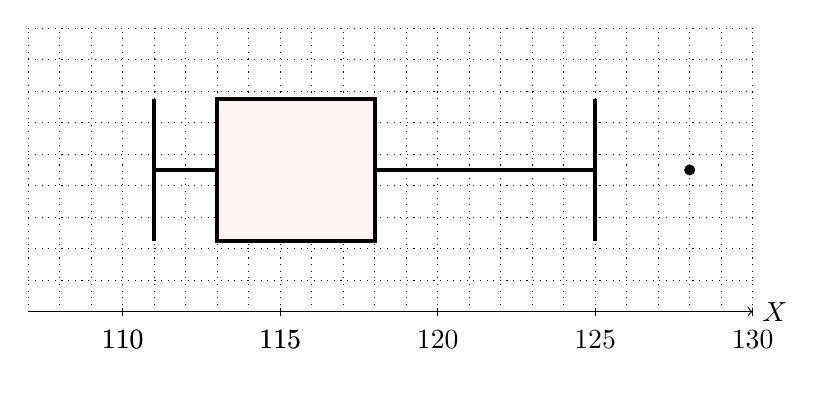
\begin{tikzpicture}[x=0.4cm,y=0.9cm]
         \draw[step=0.4cm,,dotted,color=black] (107,0) grid (130,4);
		\draw[->] (107,0) -- (130,0) node[right] {$X$} ;
		\foreach \X in {110,115,110,115,120,125,130} {
			\draw (\X,0.05cm) -- (\X,-0.05cm) node[below] {$\X\strut$};}
		\draw[ultra thick][fill=red!5] (113,1) rectangle (118,3);


		\draw[ultra thick] (111,1) -- (111,3);
		\draw[ultra thick] (111,2) -- (113,2);
		\draw[ultra thick] (118,2) -- (125,2);
		%\draw[ultra thick] (4,1) -- (4,3);
		\draw[ultra thick] (125,1) -- (125,3);
        \node[circle, fill=black, inner sep=0pt, minimum size=4pt] at (128,2) {};
			\end{tikzpicture}\\
	\end{center}

\begin{solution}
    Il manque la ligne de la médiane dans le diagramme en boîte. Les 21 données ordonnées donnent une médiane égale à la 11\textsuperscript{e} valeur, soit $\tilde{x}=115$. Il faut donc tracer un trait vertical à $x=115$ à l'intérieur de la boîte.

    On vérifie les autres éléments:
    \begin{itemize}
        \item $Q_1 = (x_{(5)}+x_{(6)})/2=(113+113)/2=113$ \checkmark
        \item $Q_3 = (x_{(16)}+x_{(17)})/2=(118+118)/2=118$ \checkmark
        \item $\text{IQR}=Q_3 - Q_1 = 5$
        \item Barrière supérieure: $Q_3+1{,}5\times\text{IQR}=118+7{,}5=125{,}5$
        \item La valeur $128 > 125{,}5$ est une valeur aberrante, correctement représentée par un point. \checkmark
        \item La moustache supérieure s'arrête à $125$, la plus grande valeur non aberrante. \checkmark
        \item La moustache inférieure s'arrête à $111$, la plus petite valeur. \checkmark
    \end{itemize}
\end{solution}
\pageblanche
\question Soit $X_1,\hdots,X_{25}$ provenant d'une loi normale d'espérance $\mu=0$ et de variance $\sigma^2=16$.

\begin{parts}
    \part[5] Quelle est la probabilité que la moyenne échantillonnale $\overline{X}$ soit égale à 0,749 fois l'écart-type échantillonnal $S$, c'est-à-dire $P(\overline{X}>0,749S)$?
    \begin{solution}
        \begin{align*}
            P(\overline{X}>0,749S)&=P(\frac{\overline{X}}{S}>0,749)\\
            &=P(\frac{\overline{X}}{S/5}>3,745)\\
            &=P(t_{24}>3,745)\\
            &=0,0005.
        \end{align*}
    \end{solution}
    \vspace{12cm}

    \part[5] Quelle est la valeur $m$, telle que la probabilité que la variance échantillonnale $S^2$ soit supérieure à $m$ est de $0,05$?
        \begin{solution}
        \begin{align*}
            P(S^2>m)&=0,05\\
            &=P(\frac{(n-1)S^2}{\sigma^2}>\frac{(n-1)m}{\sigma^2})\\
            &=P(\chi^2_{24}>\frac{24m}{16})\\
            &=0,0005.
        \end{align*}
        D'où $\frac{24m}{16}=36,42$ et $m=24,28$.
    \end{solution}
\end{parts}

\pageblanche
\end{questions}
\end{document} 
